\section{Аннотация}
В данной работе исследовано явление саморепродукции при дифракции света на периодических структурах. При помощи измерения параметров реподукции, а также с помощью геометрического увеличения и измерения пространственного спектра дифракции измерены параметры различных периодических структур: двумерных сеток разных размеров и миры из штриховых решёток. По точности измерений в каждом опыте выявлен наиболее точный метод измерений для каждого типа дифракционных решёток.

\section{Теоретические сведения}
При дифракции плоской световой волны на предмете с периодической структурой наблюдается следующее явление: на некотором расстоянии от предмета вдоль направления распространения волны появляется его изображение, периодически повторяющееся при дальнейшем движении вдоль той же оси. Это явление называется \textit{явлением саморепродукции}.

Запишем выражение для комплексной амплитуды волны, прошедшей через периодическую решётку, в плоскости, отстоящей на расстоянии $z$ от плоскости решётки:
\begin{equation*}
    f(x, z) = \sum c_ne^{i(u_nx + \sqrt{k^2-u_n^2}z)}.
\end{equation*}
Фаза $n$-ой плоской волны плоской волны в плоскости $z = \text{const}$ равна $\varphi_n = \sqrt{k^2 - u_n^2}z\approx kz - \frac{zu_n^2}{2k}$. Сравним набег фазы $n$-ой плоской волны с набегом фазы $\varphi_0$ плоской волны, бегущей вдоль оси $z$: $\varphi_0 = kz$. Получаем разность фаз
\begin{equation}\label{dphi}
    \Delta\varphi_n = \varphi_n - \varphi_0 = \frac{z}{2k}\left(\frac{2\pi}{d}\right)^2n^2 = \pi\frac{\lambda z}{d^2}n^2.
\end{equation}

Рассмотрим плоскость наблюдения, отстоящую от плоскости решётки на расстояние $z_m$, при 
\begin{equation}\label{ZZZ}
    z_m = m\frac{2d^2}{\lambda},\quad z\in\mathbb{N}.
\end{equation}
В этой плоскости из \eqref{dphi} имеем разность $\Delta\varphi_n = 2\pi m n^2$. Получаем, что разность фаз кратна $2\pi$ при любых целых $n$. Аналогично, разность фаз между любыми двумя волнами кратна $2\pi$: $\Delta\varphi_{ij} = 2\pi m(i^2-j^2)$. Получается, что фазовые соотношения между слагаемыми плоскими волнами одинаковы в плоскости решётки и в плоскости наблюдения, откуда следует, что результат интерференции этих волн также одинаков. В этом и заключается суть эффекта саморепродукции.

\section{Экспериментальная установка}
\begin{figure}[h]
    \centering
    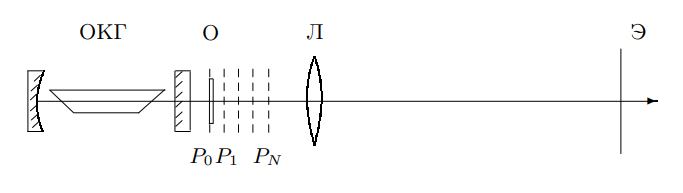
\includegraphics[width=0.7\textwidth]{img/setup.png}
    \caption{Схема установки для наблюдения саморепродукции/дифракции}
    \label{fig:setup}
\end{figure}

Хорошим приближением плоской волны в нашем эксперименте служит излучение лазера. Схема экспериментальной установки показана на рис. \ref{fig:setup}. Луч гелий-неонового лазера из генератора оптического квантового генератора (ОКГ) направляется на периодическую структуру О в плоскости $P_0$. В качестве  В плоскостях $P_1$-$P_N$ возникают изображения объекта, которые с помощью линзы Л можно поочерёдно проецировать на экран, установленный в плоскости Э.

Если убрать линзу, то на экране наблюдается картина дифракции луча лазера на периодическом объекты. Экран устанавливается достаточно далеко от объекта, так что лучи, соответствующие различным порядкам дифракции ($\sin \theta_n = n\lambda/d$), разделяются. Измеряя расстояние между дифракционными максимумами, можно определить $\sin \theta_n$ и $d$.

В качестве периодических структур в данной работе используется мира~--- набор различным образом ориентированных одномерных решёток разного период, а также набор из пяти двумерных сеток-решёток. Последние можно рассматривать как пары взаимно перпендикулярных решёток.